\documentclass{article}
\usepackage{tikz}
\usetikzlibrary{shapes,arrows}
% styles for flowcharts
\tikzstyle{machine} = [star, star points=7, star point ratio=0.8, draw, text width=5em, text badly centered, node distance=3cm, inner sep=0pt]
\tikzstyle{data} = [trapezium, trapezium left angle=70, trapezium right angle=-70, draw,text centered]
\tikzstyle{process} = [rectangle, draw, text width=5em, text centered, rounded corners, minimum height=4em] 

\addtolength{\textwidth}{10pt}

\title{Question Answering\\
\small{Project Proposal}}
\author{
Alec Story,
Ansu Abraham,
Craig Frey,\\
Dustin Tiedemann,
Michael Zhu,
Thomas Levine,
Whitney Foster\\
}

\begin{document}
\maketitle
\section{Design}

We plan to implement our question answering system in Python, and use external
tools such as the natural language toolkit.

Our design mimics the design of Watson, with the intention of trying out a
variety of techniques to select answers from documents, and to use a machine
learning system to choose the appropriate one.  See figure \ref{diagram} for
a graphical overview.

We will first analyze the question (using a parser or hand-written rules) to
determine the parts of speech a valid answer could comprise, so, for example,
``who'' questions always result in a noun phrase, and ``how'' questions usually
result in verb phrases or adverbial phrases.  We will also extract named entities
from the question.

After retrieving the documents, we search for the named entities from the
question in the documents, and return the sentences that match those entities.
These are tagged with their parts of speech, and chunked to produce all the
phrases of the appropriate type determined by analyzing the question.

These are our answer candidates.  They, and their sentence contexts, are passed
into our set of answer evaluators, which associate with them a confidence in
their accuracy.  Simple evaluators include word vector model matching against
the question, and more complex ones might include parsing, or other
sophisticated evaluation techniques.

We will then train a supervised classification algorithm to predict whether
answers are correct based on the confidence measures from the various answer
evaluation techniques. This will produce aggregate confidence measures for
each answer. Finally, we will pack the most confident answers into the 50 bytes
until we run out of space.

\begin{figure}
 \label{diagram}
 \begin{center}
  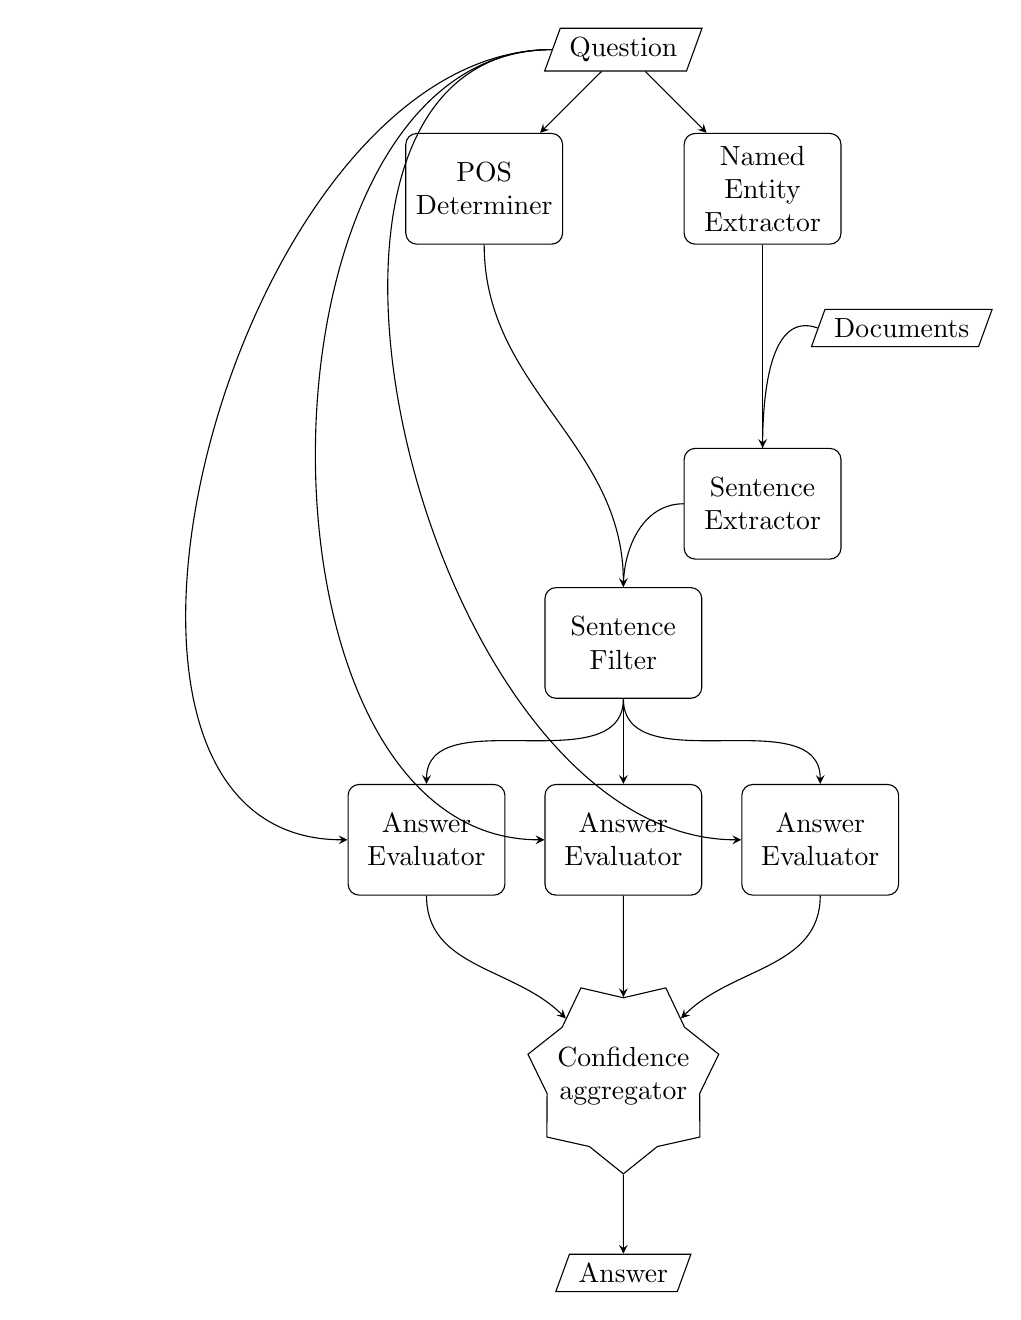
\begin{tikzpicture}[node distance=2.5cm, auto, >=stealth]
   % nodes
   \node[data] (Q)                                      {Question};
   \node[process] (pd) [below left of=Q]                {POS Determiner};
   \node[process] (na) [below right of=Q]               {Named Entity Extractor};
   \node[data] (docs) [below right of=na]               {Documents};
   \node[process] (ex) [below of=na, node distance=4cm] {Sentence Extractor};
   \node[process] (sf) [below left of=ex]               {Sentence Filter};
   \node[process] (a2) [below of=sf]                    {Answer Evaluator};
   \node[process] (a1) [left of=a2]                     {Answer Evaluator};
   \node[process] (a3) [right of=a2]                    {Answer Evaluator};
   \node[machine] (as) [below of=a2]                    {Confidence aggregator};
   \node[data] (A) [below of=as]                        {Answer};
   
   % edges
   	\draw[->] (Q) to (pd);
   	\draw[->] (Q) to (na);
   	\draw[->] (na) to (ex);
	\draw (docs.west) to [out=160, in=90] (ex);
	\draw[->] (pd.south) to [out=270, in=90] (sf);
	\draw (ex.west) to [out=180, in=90] (sf);
	\draw[->] (sf.south) to [out=270, in=90] (a1);
	\draw[->] (sf.south) to [out=270, in=90] (a2);
	\draw[->] (sf.south) to [out=270, in=90] (a3);
	\draw[->] (Q.west) to [out=180, in=180] (a1);
	\draw[->] (Q.west) to [out=180, in=180] (a2);
	\draw[->] (Q.west) to [out=180, in=180] (a3);
	\draw[->] (a1.south) to [out=270, in=135] (as);
	\draw[->] (a2.south) to [out=270, in=90] (as);
	\draw[->] (a3.south) to [out=270, in=45] (as);
	\draw[->] (as) to (A);
  \end{tikzpicture}
  \caption{Data Flow}
  \label{flowchart}
 \end{center}
\end{figure}

\section{Baseline}

Our baseline system simply takes the first answer of the training data and
repeats that as the answer to all following questions.  It is included as
\verb+zero.py+, and its mean reciprocal rank over 197 questions is 0.048.

\end{document}
